\que{Изопериметрическая задача (с доказательством).}
\subsubsection{Вариационная производная}
\begin{definition}
  Рассмотрим некоторое приращение $ h(x) $, не равно нулю лишь в некоторой
  окрестности фиксированной точки $ x_0 $. Диаметр фигуры (супремум расстояний
  между точками), ограниченной $ h(x) $ и осью $ Ox $ обозначим символом $ d(h)
  $, а её площадь со знаком (интеграл) --- символом $ \Delta s $. Тогда
  предел\footnote{Этот предел может не существовать; понятно, что $ d(h) \to 0
  \Rightarrow \Delta s \to 0 $, но обратное неверно.} \[ \left.\frac{\delta
      \mathscr J}{\delta y}\right|_{x=x_0}:=\lim_{d(h) \to 0} \frac{\mathscr J[y
      + h] - \mathscr J[y]}{\Delta s} \] и называют \emph{вариационной
      производной.} 
\end{definition}

Из определения непосредственно следует, что 
\[
  \Delta \mathscr J = \left. \frac{\delta \mathscr J}{\delta y}\right|_{x=x_0}
    \Delta s + \varepsilon(h) \Delta s,
\]
где $ \varepsilon \to 0$ при $ d(h) \to 0 $. Первое слагаемое
этого выражения называется \emph{вариацией} функционала в точке.

По тем же причинам, что и всегда, для наличия экстремума в точке $ x_0 $
требуется равенство нулю вариационной производной в этой точке.

Рассмотрим частный случай, когда  
\[
  \mathscr J[y] = \int\limits_{a}^{b}F(x, y, y')\,dx.
\]
Возьмём равномерное разбиение отрезка $ [a,b] $ с шагом $ h $. Тогда функционал
$ \mathscr J $
(при фиксированном разбиении) можно приближённо рассматривать как функцию  
\[
  J(y_1, \ldots, y_n) = \sum_{i=0}^n F\left(x_i, y_i, \frac{y_{i+1} -
  y_i}{\Delta x}\right) \Delta x.
\]
Соответственно, предел
\begin{multline*}
  \frac{\delta \mathscr J}{\delta y} := \lim_{\Delta x \to 0} \frac{\partial
  J}{\partial y_k \Delta x} = \\
  = \lim_{\Delta x \to 0} \left\{  F_y \left( x_k, y_k,
  \frac{y_{k+1} - y_j}{\Delta x} \right) - \frac{1}{\Delta x} \left[ F_{y'}
\left( x_k, y_k, \frac{y_{k+1} - y_k}{\Delta x} \right) - F_{y'} \left( x_{k-1},
y_{k-1}, \frac{y_k - y_{k-1}}{\Delta x}\right)  \right]\right\} = \\
= F_y(x, y, y') - \frac{d}{dx}F_{y'}(x, y, y')
\end{multline*}
и будем называть вариационной производной. Во-первых, заметим, что определения
действительно эквивалентны, только в данном случае $ \|h(x)\| $<<$=$>>$ \partial y_k $ уже заранее
<<бесконечно мало>> и остаётся лишь устремить $ \Delta x \to 0 $ (в данном
случае $ \Delta s $<<=>>$ \partial y_k \Delta x $), см. также рис. \ref{fig:lom}. Во-вторых, заметим, что в данном частном случае мы
получили левую часть уравнения Эйлера.
\begin{figure}[H]
  \centering
  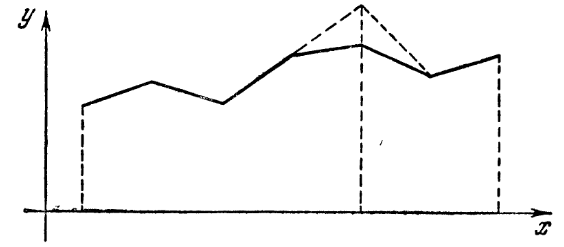
\includegraphics[width=0.8\textwidth]{img/lom.png}
  \caption{Очень вольное изображение <<площади>> $ \partial y_k\Delta x $ как
  площади фигуры между пунктирной и перманентной ломаной.}
  \label{fig:lom}
\end{figure}

\subsubsection{Изопериметрическая задача}
\begin{definition}
  \emph{Изопериметрической} называют следующую задачу. Среди всех кривых,
  удовлетворяющих условиям $ y(a) = A $, $ y(b) = B $, на которых функционал 
  \[
  \mathscr K[y] = \int\limits_{a}^{b}G(x, y, y')\,dx
  \]
принимает заданное значение $ l $, найти ту, для котой другой функционал  
\[
  \mathscr J[y] = \int\limits_{a}^{b}F(x, y, y')\,dx
\]
достигает экстремума.
\end{definition}

\textsc{Требования.}
\begin{enumerate}
  \item Функции $ G(x,y,z) $ и $ F(x,y,z)$ имеют непрерывные производные до
    второго порядка
    включительно при $ a\leqslant x \leqslant b $, $ y, z \in \mathbb R $.
  \item Искомая кривая не является экстремалью функционала $ \mathscr K $.
\end{enumerate}

\textsc{Пример.} Среди всех замкнутых кривых, имеющих заданную длину, найти
ту, которая охватывает наибольшую площадь (ответ: окружность).


\begin{theorem}
  Если кривая $ y(x) $ даёт экстремум интегралу  
  \[
    \mathscr J[y] = \int\limits_{a}^{b}F(x, y, y')\,dx,
  \]
 удовлетворяет условиям  
 \[
   \mathscr K[y] = \int\limits_{a}^{b}G(x, y, y')\,dx, \qquad y(a) = A, \quad
   y(b) = B
 \]
 и не является экстремалью функционала $ \mathscr K[y] $, то существует такая
 постоянная $ \lambda \in \mathbb R $, что кривая $ y(x) $ является экстремалью
 функционала 
 \[
     \int\limits_{a}^{b} F + \lambda G\,dx.
 \] 
\end{theorem}
\begin{proof}
  Положим, условия теоремы выполнены. Выберем приращение $ h(x) = \delta_{x_1}y
  + \delta_{x_2}y$, отличное от
  нуля лишь в окрестностях двух произвольных точек $ x_1, x_2 \in [a, b] $.
  Тогда 
  \begin{equation}\label{eq:deltaJ}
    \Delta \mathscr J = \left( \left[ F_y - \frac{d}{dx}F_{y'} \right]_{x=x_1} +
    \varepsilon_1\right)\sigma_1 + \left( \left[ F_y - \frac{d}{dx}F_{y'}
      \right]_{x=x_2} +
    \varepsilon_2\right)\sigma_2.
  \end{equation}
 Здесь  
 \[
   \sigma_1 = \int\limits_{a}^{b}\delta_{x_1}y\,dx, \quad \sigma_2 =
   \int\limits_{a}^{b}\delta_{x_2}y\,dx
 \]
 и $ \varepsilon_1, \varepsilon_2 \to 0 $ при $ \sigma_1, \sigma_2 \to 0 $.
 Такое представление следует из локальности функционала $ \mathscr J $ (а
 значит, и $ \Delta \mathscr J $).

 Кроме этого, нам необходимо потребовать, чтобы $ \mathscr K[y+h] = \mathscr K[y] = l $.
Представив $\Delta \mathscr K $ в аналогичном $ \Delta \mathscr J $ виде,
получим 
\[
        \Delta \mathscr K = \left( \left[ G_y - \frac{d}{dx}G_{y'} \right]_{x=x_1} +
    \varepsilon'_1\right)\sigma_1 + \left( \left[ G_y - \frac{d}{dx}G_{y'}
      \right]_{x=x_2} +
    \varepsilon'_2\right)\sigma_2 = 0.
\]
Выберем точку $ x_2 $ так, чтобы  
\[
  \left[ G_y - \frac{d}{dx}G_{y'} \right]_{x=x_2} \neq 0
\]
(по условию $ y(x) $ не является экстремалью функционала $ \mathscr K $!).
Тогда\footnote{Используется очевидное свойство бесконечно малых $ \frac{A +
  \alpha}{B + \beta} = \frac{A}{B} + \gamma $ для некоторой бесконечно малой $
\gamma $.}
\[
  \sigma_2 = - \left( \frac{ \left[ G_y - \frac{d}{dx} G_{y'} \right]_{x=x_1}
  }{ \left[ G_y - \frac{d}{dx}G_{y'} \right]_{x=x_2}} + \varepsilon'
\right)\sigma_1,
\]
где $ \varepsilon' \to 0 $ при $ \sigma_2 \to 0 $.

Обозначим  
\[
  \lambda = - \frac{ \left[ F_y - \frac{d}{dx}F_{y'} \right]_{x=x_2}}{ \left[
  G_y - \frac{d}{dx}G_{y'} \right]_{x=x_2}}
\]
и подставим в формулу \eqref{eq:deltaJ} вместо $ \sigma_2 $ полученное
выражение.  
\[
  \Delta \mathscr J = \left\{ \left[ F_y - \frac{d}{dx}F_{y'} \right]_{x=x_1} +
  \lambda \left[ G_y - \frac{d}{dx}G_{y'} \right]_{x=x_1}\right\}\sigma_1 +
  \varepsilon \sigma_1.
\]
Первое слагаемое есть вариация $ \mathscr J $ (относительно $h(x)$!) и при
достижении экстремума
$ \mathscr J $ вариационная производная  
\[
  F_y - \frac{d}{dx} F_{y'} + \lambda \left( G_y - \frac{d}{dx} G_{y'} \right)
  = 0
\]
 должна равняться нулю.
\end{proof}
